\documentclass[runningheads]{llncs}
%
\usepackage[T1]{fontenc}
\usepackage{graphicx}
\usepackage{booktabs}
\usepackage{amsmath}
\usepackage{amssymb}
\usepackage{array}
\usepackage{multirow}
\usepackage{xcolor}
\usepackage{hyperref}

\setlength{\textfloatsep}{5pt}
\setlength{\floatsep}{3pt}
\setlength{\intextsep}{5pt}
\setlength{\abovecaptionskip}{2pt}
\setlength{\belowcaptionskip}{1pt}
\setlength{\tabcolsep}{4pt}
\renewcommand{\arraystretch}{0.85}
\setlength{\abovedisplayskip}{4pt plus 2pt minus 2pt}
\setlength{\belowdisplayskip}{4pt plus 2pt minus 2pt}
\setlength{\abovedisplayshortskip}{2pt plus 2pt}
\setlength{\belowdisplayshortskip}{2pt plus 2pt}
\addtolength{\textwidth}{1.6cm}
\addtolength{\oddsidemargin}{-0.8cm}
\addtolength{\evensidemargin}{-0.8cm}

\begin{document}
%
\title{Trabalho Prático 1: Métodos Clássicos de Recuperação de Informação}
%
\author{Rafael Mendonça Duarte (NUSP: 16817608) \and
        João Pedro Correia Caetano (NUSP: 16987067)}
%
\authorrunning{R. M. Duarte e J. P. C. Caetano}
%
\institute{Instituto de Ciências Matemáticas e Computação -- Universidade de São Paulo\\
\email{\{rmduarte,joaopcaetanoc\}@usp.br}}
%
\maketitle
%
\begin{abstract}
Este trabalho implementa e avalia dois métodos clássicos de recuperação de informação --- o Modelo Vetorial (TF-IDF com similaridade do cosseno) e o Modelo Probabilístico BM25 --- sobre a coleção Cranfield (1400 documentos, 225 consultas, 1837 julgamentos de relevância). Quatro configurações de pré-processamento (combinando remoção de stopwords e stemming de Porter) foram comparadas para o Modelo Vetorial, e a configuração com remoção de stopwords e stemming (menor tamanho médio de documento, 104{,}4 tokens, e menor vocabulário, 6975 termos) obteve o melhor MAP em ambos os modelos, sendo adotada como padrão para as demais análises. Nessa configuração, o BM25 (MAP~=~0{,}2885) superou o Modelo Vetorial (MAP~=~0{,}2734) em todas as métricas agregadas, efeito atribuído à normalização de tamanho de documento controlada pelo parâmetro $b$. Um grid search do BM25 sobre $k_1 \in \{0{,}5;\,1{,}2;\,2{,}0\}$ e $b \in \{0;\,0{,}75;\,1\}$ identificou $k_1=2{,}0,\ b=0{,}75$ como a melhor combinação (MAP~=~0{,}2925). Análises complementares por consulta, de reformulação de consultas e de erros mostram que ambos os modelos compartilham a limitação fundamental de dependerem de sobreposição lexical exata, falhando sistematicamente diante de sinonímia e de julgamentos de relevância baseados em escopo temático.

\keywords{Recuperação de Informação \and Modelo Vetorial \and BM25 \and Cranfield \and Pré-processamento}
\end{abstract}
%
\section{Introdução}

O estudo da recuperação da informação concerne o desenvolvimento de métodos para a recuperação de dados não estruturados de acordo com uma dada consulta: um sistema de recuperação busca, em uma coleção finita de dados, quais itens são relevantes para o usuário~\cite{ref_manning}. Entre as abordagens clássicas destacam-se o Modelo Vetorial, que representa documentos e consultas como vetores ponderados por TF-IDF, e o Modelo Probabilístico, cujo expoente mais utilizado é o BM25~\cite{ref_bm25}. Ambos dependem exclusivamente de sobreposição lexical, sem noção de significado, o que os torna um ponto de partida natural para entender a eficácia e os limites de métodos estatísticos de recuperação. A coleção Cranfield, composta por resumos técnicos de aerodinâmica com julgamentos de relevância manuais, é um dos primeiros e mais tradicionais \emph{benchmarks} da área~\cite{ref_irdatasets}.

O objetivo deste trabalho é desenvolver, comparar e avaliar o Modelo Vetorial e o BM25 sobre a coleção Cranfield, usando métricas padrão de recuperação de informação, e investigar o efeito de diferentes configurações de pré-processamento, de parâmetros do BM25 e de reformulações de consulta sobre a qualidade do ranking. O restante do relatório segue: Seção~2 descreve as técnicas, Seção~3 a metodologia de avaliação, Seção~4 os resultados experimentais, e Seção~5 as considerações finais.

\vspace{-1.0em}
\section{Técnicas Utilizadas}

\subsection{Pré-processamento}

O texto foi normalizado para minúsculas e tokenizado com o \texttt{word\_tokenize} do NLTK. Quatro configurações foram comparadas, combinando (ou não) remoção de \emph{stopwords} (lista padrão de inglês do NLTK) e \emph{stemming} de Porter (\texttt{PorterStemmer}). A Tabela~\ref{tab:preproc} resume o tamanho médio de documento (tokens) e o vocabulário resultante.

\begin{table}[t]
\centering
\caption{Estatísticas de pré-processamento por configuração.}
\label{tab:preproc}
\small
\begin{tabular}{lcc}
\toprule
Configuração & Tam. médio doc. (tokens) & Vocabulário \\
\midrule
Sem remoção de stopwords, sem stemming & 170{,}83 & 9723 \\
Com remoção de stopwords, sem stemming & 104{,}39 & 9605 \\
Sem remoção de stopwords, com stemming & 170{,}83 & 7085 \\
Com remoção de stopwords, com stemming (padrão) & 104{,}39 & 6975 \\
\bottomrule
\end{tabular}
\end{table}

A remoção de stopwords reduz drasticamente o tamanho médio do documento ($-$39\%), mas quase não altera o vocabulário, pois stopwords são poucos tipos de alta frequência. Já o stemming reduz fortemente o vocabulário ($\approx$~$-$27\%) ao conflar variações morfológicas em um mesmo radical, sem afetar a contagem de tokens.

\subsection{Modelo Vetorial}

No Modelo Vetorial, documentos e consultas são representados como vetores no espaço dos termos do vocabulário, ponderados por TF-IDF. Usando o \texttt{TfidfVectorizer} do scikit-learn (tokenização por espaço em branco, pois o texto já chega pré-processado), cada peso é calculado como
\begin{equation}
\text{tfidf}(t,d) = \text{tf}(t,d) \cdot \left(\ln\frac{1+N}{1+\text{df}(t)} + 1\right),
\end{equation}
onde $\text{tf}(t,d)$ é a frequência bruta do termo $t$ em $d$, $N$ o número de documentos e $\text{df}(t)$ o número de documentos que contêm $t$ (\texttt{use\_idf=True}, \texttt{smooth\_idf=True}, \texttt{sublinear\_tf=False}). Cada vetor de documento é normalizado pela norma L2. A similaridade entre consulta $q$ e documento $d$ é o cosseno do ângulo entre seus vetores, $\cos(\vec{q},\vec{d})=\vec{q}\cdot\vec{d}/(\lVert\vec{q}\rVert\lVert\vec{d}\rVert)$, que, com os documentos normalizados, se reduz a um produto interno esparso, calculado para todos de uma vez via \texttt{cosine\_similarity}. O ranking ordena os documentos por esse score em ordem decrescente.

\vspace{-1.0em}
\subsection{Modelo Probabilístico --- BM25}

O BM25 foi implementado manualmente (sem bibliotecas externas), seguindo a formulação clássica do \emph{framework} probabilístico de relevância~\cite{ref_bm25}. O score de um documento $D$ para uma consulta $Q = \{q_1,\dots,q_n\}$ é
\begin{equation}
\text{score}(D,Q) = \sum_{i=1}^{n} \text{IDF}(q_i) \cdot \frac{f(q_i,D)\,(k_1+1)}{f(q_i,D) + k_1\left(1 - b + b\,\dfrac{|D|}{\text{avgdl}}\right)},
\end{equation}
com o IDF de Robertson calculado, por termo, como $\text{IDF}(q_i) = \ln\!\left(\frac{N - \text{df}(q_i) + 0.5}{\text{df}(q_i) + 0.5} + 1\right)$, em que $f(q_i,D)$ é a frequência de $q_i$ em $D$, $|D|$ o tamanho de $D$ em tokens e \text{avgdl} o tamanho médio dos documentos. $k_1$ controla a saturação da frequência de termo (valores altos deixam $f(q_i,D)$ crescer por mais tempo antes de saturar), enquanto $b \in [0,1]$ controla a normalização por tamanho do documento ($b=0$: sem normalização; $b=1$: normalização completa). Os parâmetros \emph{default}, salvo indicação contrária, são $k_1=1{,}2$ e $b=0{,}75$.

\vspace{-1.0em}
\section{Avaliação}

O experimento utiliza a coleção Cranfield, obtida via \texttt{ir\_datasets}~\cite{ref_irdatasets}: 1400 documentos, 225 consultas e 1837 julgamentos de relevância (\emph{qrels}). Cada qrel tem grau de 1 (interesse mínimo) a 4 (resposta completa), ou $-1$ (sem interesse); um documento é \textbf{relevante} se seu grau $\geq 1$, e não relevante caso contrário (grau $-1$ ou ausência de julgamento).

As métricas, calculadas por consulta e agregadas por média sobre as 225 consultas, são: P@10 e R@10 (fração de relevantes entre os 10 primeiros, e fração dos relevantes totais recuperada nos 10 primeiros); AP, cuja média define o MAP; F1@10, média harmônica de P@10 e R@10; RR (inverso da posição do primeiro relevante), cuja média define o MRR; e NDCG@10, que usa o grau graduado normalizado pelo DCG ideal. As configurações avaliadas foram: (i) as 4 configurações de pré-processamento no Modelo Vetorial; (ii) o BM25 padrão; (iii) um \emph{grid search} $3\times3$ de $(k_1,b)$ do BM25.

\vspace{-1.0em}
\section{Resultados e Análise}

\vspace{-1.0em}
\subsection{Comparação de pré-processamento e entre modelos}

A Tabela~\ref{tab:preproc-results} mostra as métricas do Modelo Vetorial nas quatro configurações de pré-processamento e, na última linha, o BM25 na configuração padrão (destacada), permitindo comparar de uma só vez o efeito do pré-processamento e a diferença entre modelos.

\begin{table}[t]
\centering
\caption{Métricas por configuração de pré-processamento (Vetorial) e BM25 na configuração padrão.}
\label{tab:preproc-results}
\footnotesize
\setlength{\tabcolsep}{3.5pt}
\begin{tabular}{lcccccc}
\toprule
Configuração (modelo) & MAP & P@10 & R@10 & F1@10 & MRR & NDCG@10\\
\midrule
Vet. ($-$SW, $-$St)          & 0{,}2450 & 0{,}1996 & 0{,}3198 & 0{,}2230 & 0{,}4859 & 0{,}2829\\
Vet. ($+$SW, $-$St)          & 0{,}2495 & 0{,}2093 & 0{,}3383 & 0{,}2339 & 0{,}4824 & 0{,}2919\\
Vet. ($-$SW, $+$St)          & 0{,}2646 & 0{,}2169 & 0{,}3648 & 0{,}2454 & 0{,}5033 & 0{,}3072\\
Vet. ($+$SW, $+$St, padrão)  & 0{,}2734 & 0{,}2204 & 0{,}3682 & 0{,}2490 & 0{,}5133 & 0{,}3130\\
\textbf{BM25 (padrão)} & \textbf{0{,}2885} & \textbf{0{,}2213} & \textbf{0{,}3697} & \textbf{0{,}2507} & \textbf{0{,}5249} & \textbf{0{,}3222}\\
\bottomrule
\end{tabular}
\par\vspace{1pt}\footnotesize $-$SW/$+$SW: sem/com remoção de stopwords; $-$St/$+$St: sem/com stemming.
\end{table}

A configuração com remoção de stopwords e stemming obteve o melhor MAP entre as quatro do Vetorial, sendo adotada como padrão. O stemming isoladamente traz o maior ganho (0{,}2450~$\to$~0{,}2646 sozinho; 0{,}2495~$\to$~0{,}2734 combinado): ao conflar variações morfológicas em um radical, aumenta a sobreposição exata entre termos, beneficiando precisão e revocação sem efeito colateral. A remoção de stopwords isolada traz ganho menor (0{,}2450~$\to$~0{,}2495), mas é mais relevante combinada ao stemming. Nessa configuração padrão, o BM25 supera o Vetorial em todas as métricas, com margens modestas em P@10/R@10/F1@10 ($<$~0{,}01) e mais expressivas em MAP e NDCG@10 ($\approx$~0{,}015 e~0{,}009). A explicação principal é a normalização por tamanho: o cosseno normaliza cada vetor pela norma L2 completa, podendo inflar a similaridade de documentos curtos que concentram seu peso TF-IDF em poucos termos (Seção~4.2); o BM25 usa o fator $1-b+b\,|D|/\text{avgdl}$, calibrado por $b$, um controle mais gradual.

\vspace{-1.0em}
\subsection{Análise por consulta}

Seis consultas foram selecionadas pela diferença $\text{AP}_{\text{BM25}} - \text{AP}_{\text{Vetorial}}$ na config. padrão: as 2 com maior diferença positiva (BM25 muito superior: 167, 81), as 2 com diferença mais negativa (Vetorial muito superior: 145, 77), e as 2 com pior $\max(\text{AP}_{\text{vet}},\text{AP}_{\text{bm25}})$ entre as 225 consultas (ambos insatisfatórios: 31, 22). A Tabela~\ref{tab:case-studies} traz o Top-5 de cada modelo (\checkmark\,=\,relevante).

\begin{table}[t]
\centering
\caption{Top-5 de cada modelo nas 6 consultas selecionadas.}
\label{tab:case-studies}
\scriptsize
\setlength{\tabcolsep}{3pt}
\begin{tabular}{cll}
\toprule
Q. & Vetorial --- Top-5 & BM25 --- Top-5 \\
\midrule
167 & 553, 1099, 1279, 1097, 1100 & 274\checkmark, 553, 1279, 82\checkmark, 1100 \\
81  & 714, 652, 249, 799\checkmark, 206 & 799\checkmark, 714, 672\checkmark, 631, 185 \\
145 & 1045\checkmark, 839\checkmark, 763\checkmark, 1046, 1051 & 1126, 1051, 827, 1045\checkmark, 641 \\
77  & 667\checkmark, 1264, 668\checkmark, 345, 329\checkmark & 1264, 630, 667\checkmark, 272, 345 \\
31  & 751, 68, 918, 247, 916 & 751, 1209, 1153, 1245, 1082 \\
22  & 254, 125, 560, 140, 120 & 125, 560, 413, 254, 307 \\
\bottomrule
\end{tabular}
\end{table}

Nas consultas 167 e 81 (AP Vet 0{,}108/0{,}268 vs. AP BM25 0{,}750/0{,}833), o relevante é relativamente longo (160 e 151 tokens) e contém o termo mais discriminativo (``ablat*'' na 167; ``tunnel''/``interference'' na 81); no Vetorial fica fora do Top-5, enquanto documentos mais curtos (104 e 67 tokens) sobem ao topo. Hipótese: a normalização L2 divide pelo módulo do vetor do documento inteiro, e um documento curto concentra seu peso TF-IDF em poucos termos, inflando sua similaridade; o BM25 premia o termo raro no documento correto mesmo sendo mais longo que a média.

Nas consultas 145 e 77 (AP Vet 0{,}590/0{,}545 vs. AP BM25 0{,}162/0{,}186) o padrão se inverte: o relevante da 145 é curto (18 tokens) com \emph{match} exato em três termos (``bend'', ``pressur'', ``cylind''); o cosseno o coloca em 1\textsuperscript{o}, mas o BM25 em 4\textsuperscript{o}, atrás de um não relevante 3,4$\times$ mais longo. Como o BM25 soma contribuições independentes por termo, documentos longos têm mais chance de conter \emph{algum} termo da consulta multi-termo; o cosseno recompensa a concentração temática do documento curto.

Nas consultas 31 e 22 o único relevante fica na segunda metade do ranking em ambos os modelos (doc 776: rank 1350/1400 Vet., 1375/1400 BM25; doc 68: rank 989/1400 e 1042/1400). Não há sobreposição lexical: a consulta 31 pergunta sobre ``end plate''/``aspect ratio'', e o documento relevante fala em ``cilindros quadrados e dodecagonais'' sem citar esses termos --- mismatch de vocabulário que nenhum modelo lexical resolve.

\vspace{-1.0em}
\subsection{Variação de parâmetros do BM25}

A Tabela~\ref{tab:grid} traz o MAP do grid $k_1 \in \{0{,}5;\,1{,}2;\,2{,}0\} \times b \in \{0;\,0{,}75;\,1\}$ na config. padrão.

\begin{table}[t]
\centering
\caption{MAP do BM25 por combinação $(k_1, b)$.}
\label{tab:grid}
\small
\begin{tabular}{lccc}
\toprule
$k_1 \backslash b$ & 0 & 0{,}75 & 1 \\
\midrule
0{,}5 & 0{,}2588 & 0{,}2770 & 0{,}2762 \\
1{,}2 & 0{,}2664 & 0{,}2885 & 0{,}2895 \\
2{,}0 & 0{,}2682 & \textbf{0{,}2925} & 0{,}2909 \\
\bottomrule
\end{tabular}
\end{table}

Fixando $k_1$, $b=0$ é sempre nitidamente pior que $b=0{,}75$ ou $b=1$ (ex.: $k_1=1{,}2$: MAP cai de 0{,}2885 para 0{,}2664, $-$8\%); $b=0{,}75$ e $b=1$ ficam próximos entre si (diferença~$<$~0{,}002). Fixando $b$, aumentar $k_1$ de 0{,}5 para 2{,}0 melhora o MAP consistentemente (ex.: $b=0{,}75$: 0{,}2770~$\to$~0{,}2885~$\to$~0{,}2925): como a coleção tem resumos curtos e técnicos, a repetição de um termo tende a ser sinal genuíno de foco temático, e $k_1$ maior deixa essa frequência contribuir por mais tempo antes de saturar. A melhor combinação é $k_1=2{,}0,\ b=0{,}75$ (MAP~=~0{,}2925); a pior é $k_1=0{,}5,\ b=0$ (MAP~=~0{,}2588).

Na consulta 124 (Top-10 mais alterado por $b$, $k_1=1{,}2$ fixo, só 2 documentos em comum entre os extremos), o Top-10 com $b=0$ tem documentos de 201{,}6 tokens em média --- quase o dobro de \text{avgdl}~$\approx$~104{,}4 --- caindo para 78{,}0 tokens com $b=1$. Confirma-se o esperado: sem normalização, documentos longos vencem por acumular mais ocorrências brutas; com normalização plena, documentos mais curtos que a média são favorecidos. Nenhuma das variantes traz os 4 relevantes desta consulta ao Top-10.

\begin{figure}[t]
\centering
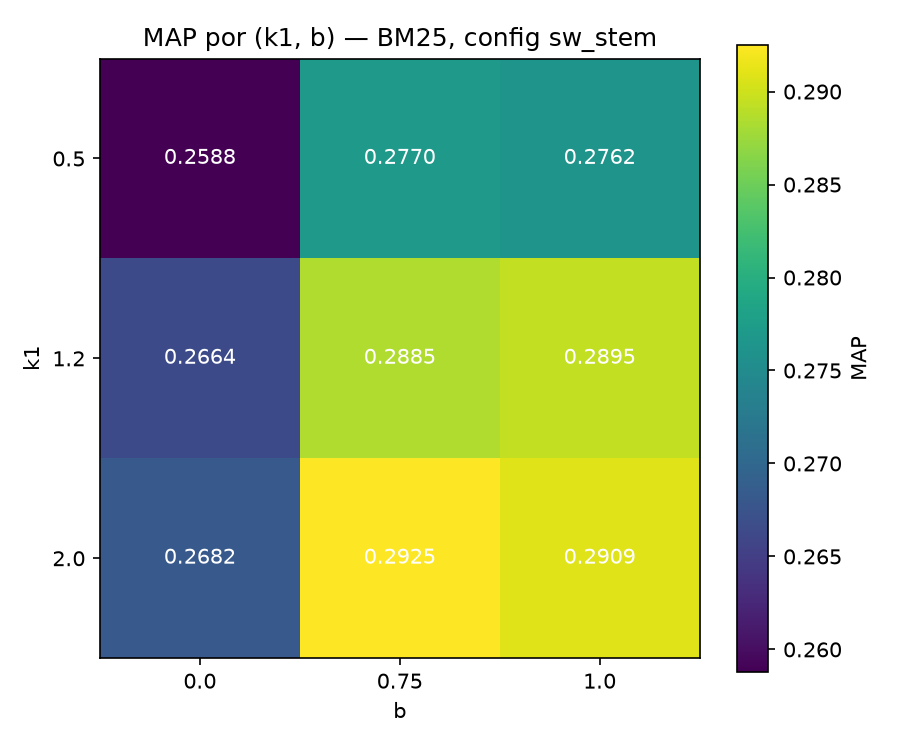
\includegraphics[width=0.5\columnwidth]{src/results/aggregated/bm25_param_heatmap.png}
\caption{MAP do BM25 por $(k_1,b)$ (config. padrão).}
\label{fig:heatmap}
\end{figure}

\vspace{-1.0em}
\subsection{Modificação de consultas}

Cinco consultas foram reformuladas manualmente (sem uso dos qrels), com estratégias de generalização, remoção/compressão de termos, sinônimo e especialização. A Tabela~\ref{tab:reform} mostra quantos dos 10 documentos do Top-10 permanecem os mesmos entre original e modificada.

\begin{table}[t]
\centering
\caption{Sobreposição do Top-10 entre consulta original e modificada.}
\label{tab:reform}
\footnotesize
\setlength{\tabcolsep}{3.5pt}
\begin{tabular}{cp{5.1cm}cc}
\toprule
Q. & Estratégia & Vet. (comuns/10) & BM25 (comuns/10) \\
\midrule
31  & Generalização (remove ``cylindrical'') & 9 & 8 \\
167 & Remoção de termos (compressão) & 8 & 7 \\
145 & Sinônimo (\emph{cylinders} $\to$ \emph{shells}) & 3 & 5 \\
100 & Especialização (acréscimo de qualificadores) & 9 & 8 \\
50  & Remoção de termos + generalização & 5 & 3 \\
\bottomrule
\end{tabular}
\end{table}

A troca por sinônimo (145) foi a mais disruptiva: no BM25, os relevantes no Top-10 caem de 2 para 0; no Vetorial, de 4 para 3. Isso ilustra a limitação central de modelos lexicais: ``cylinder''/``shell'' são sinônimos no domínio, mas após o stemming viram radicais distintos, e a troca é tratada como outro conceito. O BM25 é mais frágil a essa perda --- seu score soma contribuições independentes por termo --- enquanto o cosseno redistribui o peso entre os termos restantes. Remover/acrescentar qualificadores genéricos (31, 100) tem efeito pequeno (8--9/10 preservados), por serem termos de baixo IDF. Remover um termo de conteúdo raro (50, ``slender'') tem efeito intermediário e mais forte no BM25 (7/10 alterados) que no Vetorial (5/10), pelo mesmo motivo.

\vspace{-1.0em}
\subsection{Análise de erros}

Os falsos positivos exigem grau $-1$ explícito (não só ausência de julgamento) no rank~1 de \emph{ambos} os modelos, evitando o efeito de \emph{pooling} do Cranfield. Na consulta 3 (``heat conduction in composite slabs''), o doc.~485 (``linear heat flow in a composite slab'') tem sobreposição quase perfeita (\emph{heat, composite, slab}) mas foi julgado não relevante: a consulta pede um panorama de problemas resolvidos, o documento trata um caso específico --- diferença de escopo que nenhuma medida lexical capta. Na consulta 6, o doc.~491 compartilha vocabulário forte (\emph{turbulent, couette, flow}) mas compara o perfil do Couette a outro escoamento via lei de potência, sem fornecer os ``guias'' amplos pedidos --- mesmo problema de escopo. Como falso negativo, a consulta 124 (Seção~4.3) é, na prática, duas perguntas em uma; seu relevante mais próximo do Top-10 (doc.~967, rank~131--133/1400) compartilha vocabulário só com a primeira metade (\emph{compressible, viscous, flow}), e sua pontuação é diluída por não casar com a segunda metade da consulta.

\vspace{-1.0em}
\section{Considerações Finais}

O BM25 superou o Vetorial em todas as métricas agregadas na configuração padrão, com vantagem mais clara quando o relevante é mais longo que a média (normalização por $b$); o Vetorial se saiu melhor com relevante curto e tematicamente concentrado. A configuração mais efetiva combinou remoção de stopwords e stemming ($-$28\% de vocabulário, sem custo de desempenho). No grid do BM25, $b>0$ foi necessário e $k_1=2{,}0,\ b=0{,}75$ obteve o melhor MAP. Reformulação e erros convergem: ambos os modelos, puramente lexicais, falham diante de sinonímia e de julgamentos baseados em escopo. Limitações: tamanho pequeno e domínio específico da coleção. Extensões: expansão de consulta e modelos neurais (\emph{dense retrieval}) como \emph{baseline}.

\vspace{-1.0em}
\section{Uso de Ferramentas de IA}

O assistente de IA Claude (Anthropic) foi utilizado como apoio à programação/depuração do pré-processamento, do Vetorial e do BM25, à explicação de conceitos de RI e à escrita/formatação deste relatório. Decisões de projeto e interpretação dos resultados foram de responsabilidade dos autores.

\vspace{-1.0em}
%
\begin{thebibliography}{5}
\fontsize{8.5}{9.5}\selectfont
\setlength{\itemsep}{0pt}
\bibitem{ref_manning}
Manning, C.D., Raghavan, P., Schütze, H.: Intro. to Information Retrieval. Cambridge Univ. Press (2008)

\bibitem{ref_bm25}
Robertson, S., Zaragoza, H.: The Probabilistic Relevance Framework: BM25 and Beyond. Found. Trends Inf. Retr. \textbf{3}(4), 333--89 (2009)

\bibitem{ref_irdatasets}
ir\_datasets Documentation --- Cranfield. \url{https://ir-datasets.com/cranfield.html}

\bibitem{ref_nltk}
NLTK Project: Natural Language Toolkit Documentation. \url{https://www.nltk.org/}

\bibitem{ref_sklearn}
scikit-learn Developers: TfidfVectorizer --- API Reference. \url{https://scikit-learn.org/stable/modules/generated/sklearn.feature_extraction.text.TfidfVectorizer.html}
\end{thebibliography}

\end{document}
